\chapter{Analiza FLUENT - rețele profile separate}\label{chapter:analiza}

Pentru a ne asigura ca rezultatele obținute cu ajutorul calculelor proprii și cu ajutorul codului dezvoltat "in-house" de catedra de Mașini Hidraulice din Timișoara, dorim sa verificam rezultatele într-un software profesionale dezvoltat pentru acest fel de aplicații și anume Ansys FLUENT.

Analizam așadar rezultatele obținute prin optimizare numerica și prin analiza în FLUENT pentru coeficientul de presiune pe cele doua profile separate.

\section{Rețele profile separate. Stator}

\begin{figure}[h]
	\centering
	\includegraphics[scale=0.5]{figures/cp-stator-ezdraw.eps}
	\caption{Coeficient de presiune stator - optimizare numerică / analiză FLUENT}
	\label{Coeficient de presiune stator - optimizare numerică / analiză FLUENT}
\end{figure}

\clearpage



\section{Rețele profile separate. Rotor}

\begin{figure}[h]
	\centering
	\includegraphics[scale=0.5]{figures/cp-rotor-ezdraw.eps}
	\caption{Coeficient de presiune rotor - optimizare numerică / analiză FLUENT}
	\label{Coeficient de presiune rotor - optimizare numerică / analiză FLUENT}
\end{figure}

Se poate observa ca valorile obținute prin cele doua metode sunt extrem de apropiate, lucru care ne validează rezultatele cu un anumit grad de siguranță, fără sa avem la îndemâna o validare experimentala.

\clearpage


\section{Reprezentare analiza în tandem din FLUENT}

\begin{figure}[h]
	\centering
	\includegraphics[scale=0.5]{figures/AXENT-tandem-streamlines-ezdraw.eps}
	\caption{Reprezentare linii de curent în tandemul stator-rotor pentru turbina AXENT / analiză FLUENT}
	\label{Reprezentare linii de curent în tandemul stator-rotor pentru turbina AXENT / analiză FLUENT}
\end{figure}

Cu ajutorul FLUENT putem simula și în tandem cele doua rețele de profile, pentru a avea o imagine mai buna asupra fenomenelor hidrodinamice care apar în turbina. În figura 4.3 se pot observa liniile de curent peste cele doua profile precum și triunghiurile de viteze calculate inițial.

\clearpage